\documentclass[10pt,a4paper]{article}
\usepackage[margin=2.2cm]{geometry}
\usepackage{fontspec}
\usepackage{kotex}
\setmainfont{Apple SD Gothic Neo}
\setsansfont{Apple SD Gothic Neo}
\usepackage{amsmath,amssymb}
\usepackage{graphicx}
\usepackage{booktabs}
\usepackage{caption}
\usepackage[dvipsnames]{xcolor}
\usepackage[colorlinks=true,linkcolor=MidnightBlue,citecolor=MidnightBlue,
            urlcolor=MidnightBlue]{hyperref}
\usepackage{titlesec}
\titleformat{\section}{\large\bfseries}{\thesection}{0.6em}{}
\titleformat{\subsection}{\normalsize\bfseries}{\thesubsection}{0.5em}{}
\captionsetup{font=small,labelfont=bf}
\setlength{\parskip}{0.35em}
\setlength{\parindent}{0pt}

\usepackage{mdframed}
\newmdenv[linewidth=0.4pt,linecolor=gray!60,backgroundcolor=gray!5,
          innertopmargin=6pt,innerbottommargin=6pt,skipabove=8pt,skipbelow=8pt]{claimbox}
\newcommand{\claim}[2]{\begin{claimbox}\textbf{주장.} #1\par\smallskip
  \textcolor{gray!70}{\textbf{반증 조건.} #2}\end{claimbox}}

\title{\bfseries 이미 걸러 둔 것을 다시 걸렀다\\[2pt]
\large 원천 열 $29$개를 새 후보로 셌는데 다섯 도메인은 노트 $324$ 가 이미 걸렀다 ---
그래도 세 도메인이 남는다}
\author{월드모델 실험실 · 노트 774 · 775 · 777}
\date{2026-08-07}
\begin{document}\maketitle

\section{한 줄}

논문 $153$ 이 팝업 방문객 갈래를 내리고 T7 의 물음을 바꿨다 --- \textbf{``판의 두꺼운
도메인 원천에 아직 안 쓰는 열이 있나''}. 세었다: \textbf{$8/8$ 도메인이 문턱을 넘고
후보 $29$열.}

\textbf{그리고 그 셈이 대부분 이미 된 일이었다.} \texttt{lab/rawaxes.py} 의 머리말이
노트 $321 \cdot 324$ 의 표를 적어 두고 있었다 --- \textbf{후보 $43$개 중 출처가
$32$개($74\%$)를 막았고 그 목록에 내가 ``가장 값 있는 발견''으로 꼽은 \texttt{n\_tag}
가 있다}(\emph{``사후 의심 --- 쌓인다''}).

\textbf{그래도 남는 것이 있다} --- \texttt{rawaxes.SPEC} 이 훑은 도메인은 다섯이고
\textbf{만화 · 게임 · 도서는 없다.} 그 셋의 $11$열이 진짜 새 후보다.

\section{먼저 나온 배선 사실 --- 도메인 전용 열이 거의 없다}

판이 쓰는 특징을 찍었다. \textbf{도메인마다 $36$개이고 전 도메인이 같다.}

\begin{center}
팝업에서 온 $5$(\texttt{target\_breadth} · \texttt{venue\_prominence} ·
\texttt{entry\_friction} · \texttt{media\_push} · \texttt{goods\_scale}) $+$
\texttt{trend\_*}$3$ $+$ \texttt{cal\_*}$6$ $+$ \texttt{wiki\_*}$3$ $+$
\texttt{tag\_c*}$10$ $+$ \texttt{meta\_c*}$2$ $+$ \texttt{fund\_*}$2$ $+$
\texttt{mob\_*}$3$ $+$ \texttt{gen} · \texttt{grp}
\end{center}

\textbf{도메인 전용은 게임 $4$개뿐}(\texttt{price} · \texttt{age\_rating} ·
\texttt{ram\_gb} · \texttt{n\_category} --- 실은 앱 자료다). \textbf{즉 웹툰 · 애니 ·
만화 · 펀딩 · 세계애니에는 그 도메인만의 열이 하나도 없다.}

\begin{figure}[t]\centering
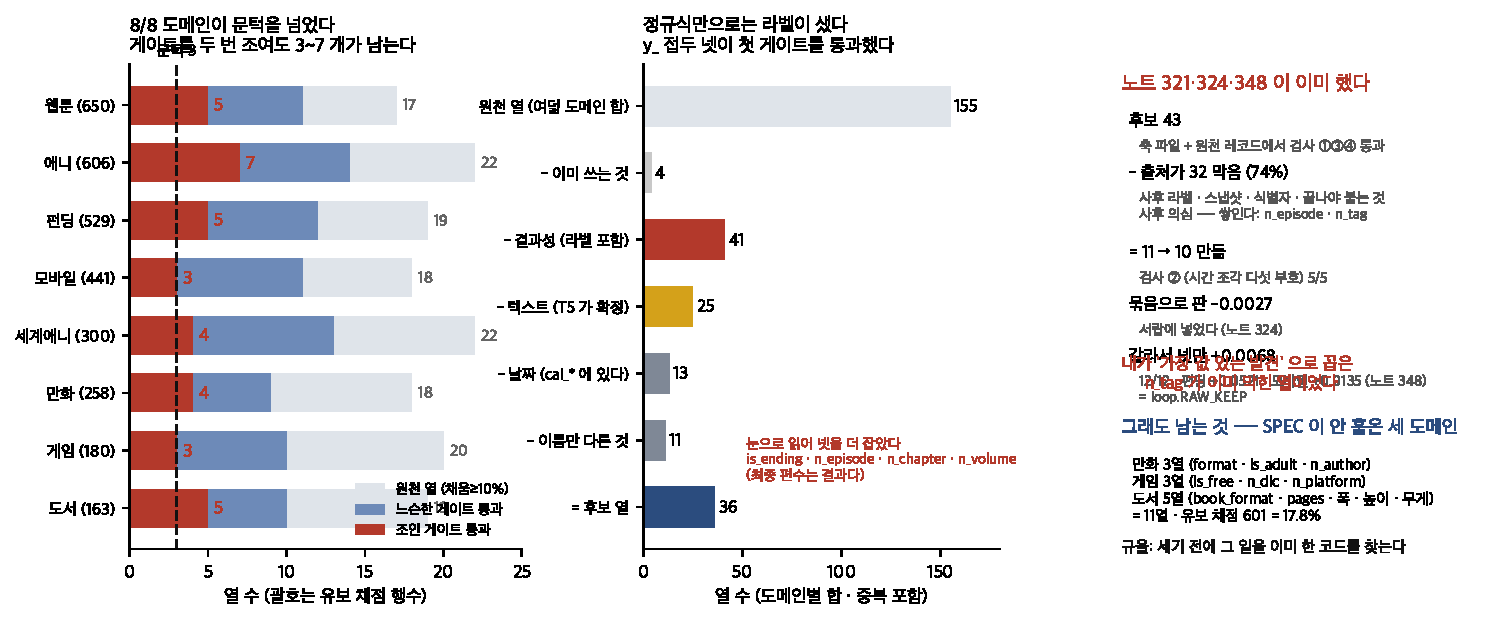
\includegraphics[width=0.99\textwidth]{figs/same29.pdf}
\caption{왼쪽: \textbf{$8/8$ 도메인이 문턱을 넘는다.} 가운데: \textbf{게이트가 무엇을
떨어뜨렸나} --- 정규식만으로는 \texttt{y\_} 접두 라벨이 샜다. 오른쪽: \textbf{그 셈이
이미 된 일이었다} --- 그리고 남는 세 도메인.}
\end{figure}

\section{세었고, 게이트를 두 번 조였다}

원천은 \texttt{data/state/\{도메인\}\_records.json} 이다.

\begin{center}
\begin{tabular}{lrrrr}
\toprule
도메인(유보) & 원천 열 & 안 쓰는 열 & 느슨한 통과 & \textbf{조인 통과} \\
\midrule
웹툰($650$) & $17$ & $17$ & $11$ & $\mathbf{5}$ \\
애니($606$) & $22$ & $21$ & $14$ & $\mathbf{7}$ \\
펀딩($529$) & $19$ & $19$ & $12$ & $\mathbf{5}$ \\
모바일($441$) & $18$ & $17$ & $11$ & $\mathbf{3}$ \\
세계애니($300$) & $22$ & $22$ & $13$ & $\mathbf{4}$ \\
만화($258$) & $18$ & $18$ & $9$ & $\mathbf{4}$ \\
게임($180$) & $20$ & $19$ & $10$ & $\mathbf{3}$ \\
도서($163$) & $19$ & $18$ & $10$ & $\mathbf{5}$ \\
\bottomrule
\end{tabular}
\end{center}

\claim{\textbf{정규식만으로는 라벨이 샌다.} 첫 게이트가 통과를 $11{\sim}15$개로 냈다.
\textbf{\texttt{y\_} 접두 라벨 넷이 통과했고}(\texttt{y\_positive} · \texttt{y\_w30} ·
\texttt{y\_favorite} · \texttt{label\_basis}) \texttt{favourites} · \texttt{amount} ·
\texttt{sale} 도 통과했다. \textbf{목록을 눈으로 읽어야 잡힌다} --- 읽어서
\texttt{is\_ending}(완결)과 \texttt{n\_episode} · \texttt{n\_chapter} ·
\texttt{n\_volume}(최종 편수는 결과다)을 더 떨어뜨렸다.}
{눈으로 읽는 것도 놓친다 --- 그것이 다음 절이다. \textbf{내가 눈으로 읽고도
\texttt{n\_tag} 를 통과시켰고, 저장소는 그것을 이미 막아 뒀다.}}

\textbf{떨어뜨린 갈래}: 결과성(라벨 포함) · \textbf{텍스트}(T5 가 ``도메인 안 전용''으로
확정 · 노트 $719 \cdot 729$) · \textbf{날짜}(\texttt{cal\_*} 여섯 열에 있다) ·
\textbf{이름만 다른 것}(\texttt{max\_price}$=$\texttt{fund\_maxprice} ·
\texttt{n\_lang}$=$\texttt{mob\_nlang} · \texttt{advisory}$=$\texttt{mob\_advisory} 등).

\section{그리고 그 셈이 이미 된 일이었다}

\texttt{lab/rawaxes.py} 를 읽었다. \textbf{머리말이 표를 적어 두고 있었다.}

\begin{center}
\begin{tabular}{lr l}
\toprule
후보 & $43$ & 축 파일 $+$ 원천 레코드에서 검사 ①③④ 통과(노트 $321 \cdot 324$) \\
$-$ 출처가 막음 & $\mathbf{32}$ & $74\%$ --- 사후 라벨 · 지금 긁은 스냅샷 · 식별자 · \\
& & 끝나야 붙는 것 · \textbf{사후 의심으로 쌓이는 것}(\texttt{n\_episode} · \textbf{\texttt{n\_tag}}) \\
$=$ 남은 것 & $11$ & 그중 \textbf{$10$}이 검사 ②(시간 조각 다섯 부호 일치) $5/5$ \\
\midrule
묶음으로 판 & $\mathbf{-0.0027}$ & \textbf{서랍에 넣었다}(노트 $324$) \\
갈라서 넷만 & $\mathbf{+0.0068}$ & $12/12$ · 펀딩 $+0.0521$ · 모바일 $+0.0135$(노트 $348$) \\
& & $=$ \texttt{loop.RAW\_KEEP} \\
\bottomrule
\end{tabular}
\end{center}

\claim{\textbf{내가 ``가장 값 있는 발견''으로 꼽은 열이 이미 막힌 열이었다.}
\texttt{n\_tag} 는 \emph{``사후 의심 --- 쌓인다''} 로 분류돼 있다. 나는 그것을 두고
\emph{``$4$ 도메인에 이름이 같아 T5 가 찾던 공유할 것의 후보''}라고 적었다. \textbf{규율:
후보를 세기 전에 그 후보를 이미 걸러 둔 코드를 찾는다.} 노트 $763$(\emph{``기제를
세우기 전에 채점 규칙을 읽는다''})의 짝이고 \textbf{이 계열이 이 세션에서 세
번째다} --- 노트 $738$(가드의 시험대를 안 적음) · 노트 $763$(채점 규칙을 안 읽음) ·
여기(이미 한 셈을 다시 함).}
{다시 센 것이 완전한 낭비는 아니다 --- \textbf{배선 사실 하나}(판 특징 $36$개가 전
도메인 동일 · 전용 열이 게임 $4$개뿐)와 \textbf{안 훑은 세 도메인}이 그 덕에 나왔다.
\textbf{그러나 그 둘은 \texttt{rawaxes.py} 를 먼저 읽었어도 나왔을 것이고, 더 빨리
나왔을 것이다.}}

\subsection*{노트 348 의 교훈을 되찾았다}

\begin{center}
\textbf{묶음으로는 못 쓰고 갈라면 쓴다} --- 지는 여섯이 이기는 넷을 덮고 있었다.
\end{center}

\textbf{이것은 논문 $146$ 이 잰 것과 같은 층이다} --- 열을 많이 넣는 것이 싸다는 것과
\emph{도움 되는 열만 골라야} 한다는 것은 다른 문장이다. 그리고 논문 $144$ 가
\textbf{소스 고르기는 잡음 예산 안에서만 이득}임을 쟀다. \textbf{여기서는 고르기가
$-0.0027 \to +0.0068$ 을 냈다} --- 도메인이 클러스터이고 클러스터가 $12$개라 고르기의
잡음이 작았기 때문이다.

\section{그래도 세 도메인이 남는다}

\texttt{rawaxes.SPEC} 의 도메인은 \textbf{모바일 · 웹툰 · 애니 · 세계애니 · 펀딩
다섯}이다. \textbf{만화 · 게임 · 도서는 없다.}

\begin{center}
\begin{tabular}{lll}
\toprule
만화($258$) & \texttt{format} · \texttt{is\_adult} · \texttt{n\_author} & $3$열 \\
게임($180$) & \texttt{is\_free} · \texttt{n\_dlc} · \texttt{n\_platform} & $3$열 \\
도서($163$) & \texttt{book\_format} · \texttt{pages} · \texttt{width\_mm} · \texttt{height\_mm} · \texttt{weight\_g} & $5$열 \\
\midrule
& \textbf{$11$열 · 유보 채점 $601$ $=$ 판 유보의 $17.8\%$} & \\
\bottomrule
\end{tabular}
\end{center}

\claim{\textbf{도서의 물리 치수가 가장 깨끗하다.} 쪽수 · 판형 · 폭 · 높이 · 무게는
\textbf{출간 시점에 확정}되고 \textbf{인기와 함께 자라지 않는다} ---
\texttt{n\_tag} 가 막힌 이유가 정확히 ``쌓인다''였다. \textbf{그리고 그것은 지금까지 이
판이 한 번도 안 써 본 종류의 정보다}(물리적 형태).}
{도서는 유보 $163$행으로 얇다 --- 논문 $146$ 이 \textbf{얇은 도메인에서 열당 비용이
$0.02{\sim}0.025$}라고 적었으므로 $5$열은 그 도메인에서 비쌀 수 있다. \textbf{그래서
노트 $348$ 의 순서를 지켜 도메인별로 갈라 넣고, 그 도메인 점수가 위약을 이기는지를
먼저 본다.}}

\subsection*{다음 실험을 값으로 적었다}

\begin{center}
\begin{tabular}{ll}
\toprule
\textbf{갑(만들기)} & 세 도메인 $11$열을 \texttt{rawaxes} 관례로 축으로 만든다 \\
& 범주형은 집단 크기 순 $0{\sim}1$ · $20$건 미만 마스크 $0$ · 수치형은 관측값만 백분위 \\
& \textbf{라벨을 한 번도 안 본다} \\
\midrule
\textbf{을(재기)} & 🔴 \textbf{묶음으로 넣지 않는다}(노트 $348$) --- 도메인 하나씩 그 도메인 열만 \\
& 위약 $3$ 뽑기(규약 $20$) · 씨앗 $6$ · 창 안 백분위(규약 $27$) · 유보 덮음률 $1.000$(규약 $22$) \\
\midrule
\textbf{판정} & 그 도메인 점수가 위약 $3$ 뽑기 전부보다 크고 판이 문턱 안에서 안 나빠지면 남긴다 \\
& \textbf{셋 다 지면 원천이 말랐고 외부 API 가 유일한 길이다} \\
\bottomrule
\end{tabular}
\end{center}

\textbf{그리고 \texttt{n\_tag} 는 안 쓴다.}

\end{document}
